% quiz.tex -- Module 5 Topic 3 (gravity): 30 new multiple-choice questions in the
% Questions 1-6 force and field, 7-18 orbits and Kepler's laws, 19-30 energy and
% Key: 1C 2D 3A 4B 5D 6C 7A 8D 9D 10B 11C 12D 13A 14C 15A
%      16B 17C 18D 19A 20B 21C 22D 23B 24C 25A 26C 27A 28B 29D 30B
% Every number: checks/m5t3-booklet/numbers.py
% Build: TEXINPUTS=.: xelatex quiz.tex (twice)
\documentclass[12pt]{article}
\usepackage{quiz}
\hypersetup{pdftitle={Multiple Choice Quiz - Module 5 Topic 3 - Gravity}}

\begin{document}
\quiztitle{Year 12 Physics}{Multiple Choice Quiz - Module 5 Topic 3 - Gravity}

% ---- Q1 (Newton's third law)
\begin{quizq}{}
A satellite of mass \qty{1000}{kg} orbits Earth. Which statement about the gravitational forces
between Earth and the satellite is correct?
\opts{Earth pulls on the satellite with a bigger force than the satellite pulls on Earth.}
  {The satellite does not pull on Earth, because its mass is too small.}
  {The two forces are equal in size, but Earth's acceleration is much smaller than the
   satellite's acceleration.}
  {The two forces are equal in size, so Earth and the satellite have equal accelerations.}
\end{quizq}

% ---- Q2 (g from mass and radius ratios)
\Needspace{11\baselineskip}
\begin{quizq}{}
Planet P has 2 times the mass of Earth and half the radius of Earth.

What is the magnitude of the gravitational field strength at the surface of planet P?
\opts{$\dfrac{1}{2}\,g$}{$2\,g$}{$4\,g$}{$8\,g$}
\end{quizq}

% ---- Q3 (altitude where g is one-ninth)
\Needspace{12\baselineskip}
\begin{quizq}{}
The gravitational field strength at Earth's surface is $g$. The radius of Earth is $r_\mathrm{E}$.

At what altitude (height above Earth's surface) is the gravitational field strength equal to
$\dfrac{g}{9}$?
\opts{$2\,r_\mathrm{E}$}{$3\,r_\mathrm{E}$}{$8\,r_\mathrm{E}$}{$9\,r_\mathrm{E}$}
\end{quizq}

% ---- Q4 (force of Mars on Phobos)
\Needspace{17\baselineskip}
\begin{quizq}{}
\renewcommand\arraystretch{1.6}
\begin{tabular}{|p{80mm}|>{\raggedleft\arraybackslash}p{36mm}|}
  \hline
  Orbital period of Phobos around Mars & \qty{2.75e4}{s}\\ \hline
  Mean orbital radius of Phobos & \qty{9.38e6}{m}\\ \hline
  Mass of Mars & \qty{6.42e23}{kg}\\ \hline
  Mass of Phobos & \qty{1.07e16}{kg}\\ \hline
\end{tabular}

What is the gravitational force that Mars exerts on Phobos?
\opts{\qty{0.49}{N}}{\qty{5.2e15}{N}}{\qty{5.2e21}{N}}{\qty{4.9e22}{N}}
\end{quizq}

% ---- Q5 (pendulum on Earth and the Moon: T^2 against l)
\Needspace{40\baselineskip}
\begin{quizq}{}
A pendulum can be used to determine the acceleration due to gravity using the relationship
\[ T = 2\pi\sqrt{\frac{l}{g}} \]
where $T$ is the period and $l$ is the length of the pendulum.

The acceleration due to gravity on the surface of the Moon is about one-sixth of that on Earth.

A student plots $T^2$ (vertical axis) against $l$ (horizontal axis) for both. Which graph relates
the variables for the pendulum correctly for both the Earth and the Moon?
\begin{center}
  \begin{tabular}{@{}l@{}}
    \textsf{\headfont\bfseries KEY}\\[2pt]
    \begin{tabular}{|l|}
      \hline
      \tikz[baseline=-0.6ex]\draw[line width=0.8pt] (0,0) -- (1.4,0);\quad Earth data\\
      \tikz[baseline=-0.6ex]\draw[line width=0.8pt, dash pattern=on 3pt off 2pt] (0,0) -- (1.4,0);\quad Moon data\\
      \hline
    \end{tabular}
  \end{tabular}
\end{center}
\gridopts{%
  \begin{tikzpicture}
    \draw[axisline] (0,0) -- (3.0,0); \draw[axisline] (0,0) -- (0,2.2);
    \node[font=\bfseries\small, left] at (0,1.15) {$T^2$};
    \node[font=\bfseries\small, below] at (1.5,0) {Length};
    \draw[line width=0.8pt] (0,0) -- (2.6,1.85);
    \draw[line width=0.8pt, dash pattern=on 3pt off 2pt] (0,0) -- (2.6,0.35);
  \end{tikzpicture}}
  {%
  \begin{tikzpicture}
    \draw[axisline] (0,0) -- (3.0,0); \draw[axisline] (0,0) -- (0,2.2);
    \node[font=\bfseries\small, left] at (0,1.15) {$T^2$};
    \node[font=\bfseries\small, below] at (1.5,0) {Length};
    \draw[line width=0.8pt, domain=0:2.6, samples=60, smooth] plot (\x, {0.22*sqrt(\x)});
    \draw[line width=0.8pt, dash pattern=on 3pt off 2pt, domain=0:2.6, samples=60, smooth] plot (\x, {1.15*sqrt(\x)});
  \end{tikzpicture}}
  {%
  \begin{tikzpicture}
    \draw[axisline] (0,0) -- (3.0,0); \draw[axisline] (0,0) -- (0,2.2);
    \node[font=\bfseries\small, left] at (0,1.15) {$T^2$};
    \node[font=\bfseries\small, below] at (1.5,0) {Length};
    \draw[line width=0.8pt, domain=0:2.6, samples=60, smooth] plot (\x, {1.15*sqrt(\x)});
    \draw[line width=0.8pt, dash pattern=on 3pt off 2pt, domain=0:2.6, samples=60, smooth] plot (\x, {0.22*sqrt(\x)});
  \end{tikzpicture}}
  {%
  \begin{tikzpicture}
    \draw[axisline] (0,0) -- (3.0,0); \draw[axisline] (0,0) -- (0,2.2);
    \node[font=\bfseries\small, left] at (0,1.15) {$T^2$};
    \node[font=\bfseries\small, below] at (1.5,0) {Length};
    \draw[line width=0.8pt] (0,0) -- (2.6,0.35);
    \draw[line width=0.8pt, dash pattern=on 3pt off 2pt] (0,0) -- (2.6,1.85);
  \end{tikzpicture}}
\end{quizq}

% ---- Q6 (point where the net force is zero, Earth-Moon)
\Needspace{15\baselineskip}
\begin{quizq}{}
The mass of Earth is about 81 times the mass of the Moon. A spacecraft travels in a straight line
from Earth to the Moon. At one point on this line, the net gravitational force on the spacecraft
is zero.

Where is this point? (Distances are measured between centres.)
\opts{Halfway between Earth and the Moon}
  {$\frac{1}{10}$ of the way from Earth to the Moon}
  {$\frac{9}{10}$ of the way from Earth to the Moon}
  {$\frac{81}{82}$ of the way from Earth to the Moon}
\end{quizq}

% ---- Q7 (forces on a satellite in a stable circular orbit)
\Needspace{38\baselineskip}
\begin{quizq}{}
Which of the following diagrams correctly represents the force(s) acting on a satellite in a
stable circular orbit around Earth?

\renewcommand\arraystretch{1.4}
\begin{tabular}{|p{68mm}p{72mm}|}
  \hline
  $F_\mathrm{g}$ = gravitational force & $F_\mathrm{p}$ = propulsive force (engine thrust)\\
  $F_\mathrm{c}$ = centripetal force & \\
  \hline
\end{tabular}
\gridopts{%
  \begin{tikzpicture}
    \path (-1.8,-1.55) rectangle (1.8,2.25);
    \shade[ball color=black!25] (0,0) circle (0.75);
    \draw[force] (0,1.5) -- (0,0.92) node[pos=0.6, left] {$F_\mathrm{g}$};
    \draw[object] (-0.18,1.42) rectangle (0.18,1.58);
  \end{tikzpicture}}
  {%
  \begin{tikzpicture}
    \path (-1.8,-1.55) rectangle (1.8,2.25);
    \shade[ball color=black!25] (0,0) circle (0.75);
    \draw[force] (0,1.5) -- (0,0.92) node[pos=0.6, left] {$F_\mathrm{g}$};
    \draw[force] (0,1.5) -- (0,2.18) node[pos=0.7, left] {$F_\mathrm{c}$};
    \draw[object] (-0.18,1.42) rectangle (0.18,1.58);
  \end{tikzpicture}}
  {%
  \begin{tikzpicture}
    \path (-1.8,-1.55) rectangle (1.8,2.25);
    \shade[ball color=black!25] (0,0) circle (0.75);
    \draw[force] (0,1.5) -- (0,0.92) node[pos=0.6, left] {$F_\mathrm{g}$};
    \draw[force] (0,1.5) -- (0.85,1.5) node[above] {$F_\mathrm{p}$};
    \draw[object] (-0.18,1.42) rectangle (0.18,1.58);
  \end{tikzpicture}}
  {%
  \begin{tikzpicture}
    \path (-1.8,-1.55) rectangle (1.8,2.25);
    \shade[ball color=black!25] (0,0) circle (0.75);
    \draw[force] (-0.1,1.5) -- (-0.1,0.92) node[pos=0.6, left] {$F_\mathrm{g}$};
    \draw[force] (0.1,1.5) -- (0.1,0.92) node[pos=0.6, right] {$F_\mathrm{c}$};
    \draw[object] (-0.18,1.42) rectangle (0.18,1.58);
  \end{tikzpicture}}
\end{quizq}

% ---- Q8 (geostationary orbit)
\Needspace{14\baselineskip}
\begin{quizq}{}
Which statement about a geostationary satellite is correct?
\opts{It can stay above any point on Earth, for example above Sydney.}
  {It has a lower altitude than a satellite in low Earth orbit.}
  {It moves faster than a satellite in low Earth orbit.}
  {It orbits above the equator, in the same direction as Earth spins, with a period of about
   24 hours.}
\end{quizq}

% ---- Q9 (two satellites in the same orbit, different masses)
\Needspace{13\baselineskip}
\begin{quizq}{}
Two satellites share a circular orbit around Earth. One satellite has three times the mass of the
other.

Which quantity would be the \emph{same} for the two satellites?
\opts{Kinetic energy}{Gravitational force}{Gravitational potential energy}{Orbital speed}
\end{quizq}

% ---- Q10 (orbital speed when r becomes 9r)
\Needspace{14\baselineskip}
\begin{quizq}{}
A satellite in circular orbit at a distance $r$ from the centre of a planet has an orbital
velocity $v$.

If the distance was increased to $9r$, what would be the satellite's orbital velocity?
\opts{$\dfrac{v}{9}$}{$\dfrac{v}{3}$}{$3v$}{$9v$}
\end{quizq}

% ---- Q11 (period when r becomes 4r)
\Needspace{12\baselineskip}
\begin{quizq}{}
A moon orbits a planet in a circular orbit with period $T$. A second moon orbits the same planet
with an orbital radius 4 times as large.

What is the period of the second moon?
\opts{$2T$}{$4T$}{$8T$}{$16T$}
\end{quizq}

% ---- Q12 (which graph is a straight line)
\Needspace{13\baselineskip}
\begin{quizq}{}
For satellites in circular orbits around the same planet, $\dfrac{r^3}{T^2} = \dfrac{GM}{4\pi^2}$.

Which graph would give a straight line through the origin?
\opts{$T$ (vertical axis) against $r$ (horizontal axis)}
  {$T$ (vertical axis) against $r^3$ (horizontal axis)}
  {$T^2$ (vertical axis) against $r$ (horizontal axis)}
  {$T^2$ (vertical axis) against $r^3$ (horizontal axis)}
\end{quizq}

% ---- Q13 (Kepler's second law, equal areas)
% Ellipse a = 3, b = 2.4, e = 0.6, star at the focus (1.8, 0). The shaded sectors have equal
% areas: E from -0.5 to 0.5 rad and from pi-0.1328 to pi+0.1328 rad.
\Needspace{34\baselineskip}
\begin{quizq}{}
The diagram shows the elliptical orbit of a planet around a star. The two shaded areas are equal.
The planet takes 40 days to move from $P_1$ to $P_2$.
\begin{center}
  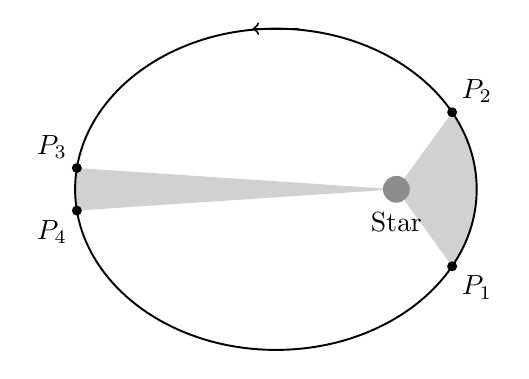
\begin{tikzpicture}[x=0.85cm, y=0.85cm]
    \fill[black!18] (1.8,0) -- plot[domain=-0.5:0.5, samples=30, smooth]
      ({3*cos(\x r)}, {2.4*sin(\x r)}) -- cycle;
    \fill[black!18] (1.8,0) -- plot[domain=3.0088:3.2744, samples=10, smooth]
      ({3*cos(\x r)}, {2.4*sin(\x r)}) -- cycle;
    \draw[line width=0.7pt] (0,0) ellipse (3 and 2.4);
    \draw[->, line width=0.7pt] (0.35,2.4) -- (-0.35,2.4);
    \fill[black!45] (1.8,0) circle (0.2);
    \node[below=5pt] at (1.8,0) {Star};
    \fill (2.633,-1.151) circle (1.8pt) node[below right] {$P_1$};
    \fill (2.633,1.151) circle (1.8pt) node[above right] {$P_2$};
    \fill (-2.974,0.318) circle (1.8pt) node[above left] {$P_3$};
    \fill (-2.974,-0.318) circle (1.8pt) node[below left] {$P_4$};
  \end{tikzpicture}
\end{center}
Which statement is correct?
\opts{It takes 40 days to move from $P_3$ to $P_4$. The planet moves faster between $P_1$ and
   $P_2$.}
  {It takes 40 days to move from $P_3$ to $P_4$. The planet moves faster between $P_3$ and $P_4$.}
  {It takes more than 40 days to move from $P_3$ to $P_4$. The planet moves faster between $P_1$
   and $P_2$.}
  {It takes less than 40 days to move from $P_3$ to $P_4$. The planet moves faster between $P_3$
   and $P_4$.}
\end{quizq}

% ---- Q14 (Kepler's third law in AU and years)
\Needspace{14\baselineskip}
\begin{quizq}{}
A dwarf planet orbits the Sun with a period of 125 years.

The average distance from the Sun to Earth is one astronomical unit.

What is the average distance between this dwarf planet and the Sun in astronomical units?
\opts{5.0}{11}{25}{1400}
\end{quizq}

% ---- Q15 (orbital speed of the ISS)
\Needspace{12\baselineskip}
\begin{quizq}{}
The International Space Station (ISS) orbits Earth in a circular orbit at an altitude of
\qty{420}{km}. What is its orbital speed?
\opts{\qty{7.68e3}{m.s^{-1}}}{\qty{7.93e3}{m.s^{-1}}}{\qty{1.09e4}{m.s^{-1}}}
  {\qty{3.09e4}{m.s^{-1}}}
\end{quizq}

% ---- Q16 (altitude of a geostationary satellite)
\Needspace{12\baselineskip}
\begin{quizq}{}
A geostationary satellite has an orbital period of 24.0 hours. What is its altitude above Earth's
surface?
\opts{\qty{1.80e5}{m}}{\qty{3.59e7}{m}}{\qty{4.23e7}{m}}{\qty{7.57e22}{m}}
\end{quizq}

% ---- Q17 (mass of Jupiter from Io)
\Needspace{12\baselineskip}
\begin{quizq}{}
Io is a moon of Jupiter. Its orbit is close to a circle, with radius \qty{4.22e8}{m} and period
\qty{1.53e5}{s}. What is the mass of Jupiter?
\opts{\qty{4.50e18}{kg}}{\qty{4.81e25}{kg}}{\qty{1.90e27}{kg}}{\qty{2.91e32}{kg}}
\end{quizq}

% ---- Q18 (T^2 against r^3 for the moons of two planets)
\Needspace{30\baselineskip}
\begin{quizq}{}
The graph shows $T^2$ against $r^3$ for the moons of two planets, X and Y.
\begin{center}
  \begin{tikzpicture}
    \draw[axisline] (0,0) -- (4.4,0) node[below left] {$r^3$};
    \draw[axisline] (0,0) -- (0,3.0) node[above] {$T^2$};
    \draw[line width=0.8pt] (0,0) -- (2.4,2.6) node[right] {Planet X};
    \draw[line width=0.8pt, dash pattern=on 3pt off 2pt] (0,0) -- (3.8,1.5) node[right] {Planet Y};
    \foreach \x/\y in {0.6/0.65, 1.2/1.3, 1.8/1.95, 0.9/0.355, 1.9/0.75, 2.85/1.125}
      {\fill (\x,\y) circle (1.8pt);}
  \end{tikzpicture}
\end{center}
Which statement is correct?
\opts{Planet X has the greater mass, because its line is steeper.}
  {The two planets have the same mass, because both lines pass through the origin.}
  {The masses cannot be compared, because the moons have different masses.}
  {Planet Y has the greater mass, because its line is less steep.}
\end{quizq}

% ---- Q19 (comet in an elliptical orbit)
\Needspace{24\baselineskip}
\begin{quizq}{}
The elliptical orbit of a comet around a star is shown.
\begin{center}
  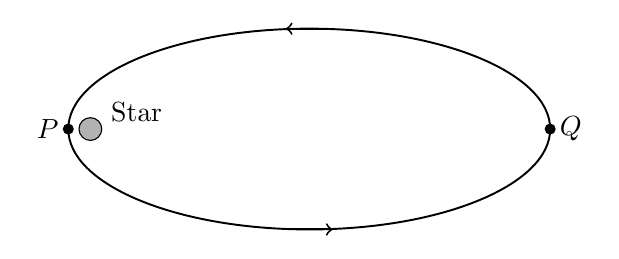
\begin{tikzpicture}[x=0.85cm, y=0.85cm]
    \draw[line width=0.7pt] (0,0) ellipse (3.6 and 1.5);
    \draw[->, line width=0.7pt] (0.35,1.5) -- (-0.35,1.5);
    \draw[->, line width=0.7pt] (-0.35,-1.5) -- (0.35,-1.5);
    \fill[black!30] (-3.27,0) circle (0.17); \draw (-3.27,0) circle (0.17);
    \node[right=4pt] at (-3.27,0.25) {Star};
    \fill (-3.6,0) circle (2pt) node[left] {$P$};
    \fill (3.6,0) circle (2pt) node[right] {$Q$};
  \end{tikzpicture}
\end{center}
Which quantity is greater at position $Q$ than at $P$?
\opts{Gravitational potential energy}{Kinetic energy}{Speed}{Total energy}
\end{quizq}

% ---- Q20 (elliptical orbit: speed and total energy)
\Needspace{32\baselineskip}
\begin{quizq}{}
A satellite orbits Earth with an elliptical orbit that passes through positions $X$ and $Y$.
\begin{center}
  \begin{tikzpicture}[x=0.85cm, y=0.85cm]
    \draw[guide, line width=0.7pt] (0,0) ellipse (3.6 and 2.0);
    \shade[ball color=black!25] (-2.75,0) circle (0.55);
    \node[font=\footnotesize] at (-2.75,0) {Earth};
    \fill (-3.6,0) circle (2pt) node[left] {$X$};
    \fill (3.6,0) circle (2pt) node[right] {$Y$};
  \end{tikzpicture}
\end{center}
Which row of the table correctly identifies the position at which the satellite has greater speed
and the position at which it has greater total energy (kinetic + potential)?
\begin{center}
  \renewcommand\arraystretch{1.7}
  \begin{tabular}{@{}p{10mm}|>{\centering\arraybackslash}p{38mm}|>{\centering\arraybackslash}p{48mm}|}
    \cline{2-3}
    & \textit{Greater speed} & \textit{Greater total energy}\\ \cline{2-3}
    A. & $X$ & $X$\\ \cline{2-3}
    B. & $X$ & Same at $X$ and $Y$\\ \cline{2-3}
    C. & $Y$ & $Y$\\ \cline{2-3}
    D. & $Y$ & Same at $X$ and $Y$\\ \cline{2-3}
  \end{tabular}
\end{center}
\end{quizq}

% ---- Q21 (LEO and GEO: potential energy and speed)
\Needspace{22\baselineskip}
\begin{quizq}{}
Two satellites have the same mass. One (LEO) is in low-Earth orbit and the other (GEO) is in a
geostationary orbit.

Which row of the table correctly identifies the satellite with the greater gravitational
potential energy and the satellite with the greater orbital speed?
\begin{center}
  \renewcommand\arraystretch{1.7}
  \begin{tabular}{@{}p{10mm}|>{\centering\arraybackslash}p{60mm}|>{\centering\arraybackslash}p{44mm}|}
    \cline{2-3}
    & \textit{Greater gravitational potential energy} & \textit{Greater orbital speed}\\ \cline{2-3}
    A. & LEO & LEO\\ \cline{2-3}
    B. & LEO & GEO\\ \cline{2-3}
    C. & GEO & LEO\\ \cline{2-3}
    D. & GEO & GEO\\ \cline{2-3}
  \end{tabular}
\end{center}
\end{quizq}

% ---- Q22 (moving to a higher orbit)
\Needspace{13\baselineskip}
\begin{quizq}{}
A satellite is moved from a low circular orbit to a higher circular orbit around Earth. Which
statement about the orbit change is correct?
\opts{Its kinetic energy increases.}{Its gravitational potential energy decreases.}
  {Its orbital period decreases.}{Its total energy increases.}
\end{quizq}

% ---- Q23 (potential energy of a satellite)
\Needspace{12\baselineskip}
\begin{quizq}{}
The gravitational potential energy of a satellite with mass \qty{1.20e3}{kg} when orbiting Earth at
an altitude of \qty{3.50e3}{km} is closest to:
\opts{\qty{-2.43e10}{J}}{\qty{-4.87e10}{J}}{\qty{-7.54e10}{J}}{\qty{-1.37e11}{J}}
\end{quizq}

% ---- Q24 (change in U read from a graph; m = 200 kg)
\Needspace{42\baselineskip}
\begin{quizq}{}
The graph shows how the gravitational potential energy ($U$) of a \qty{200}{kg} satellite changes
with its altitude.
\begin{center}
  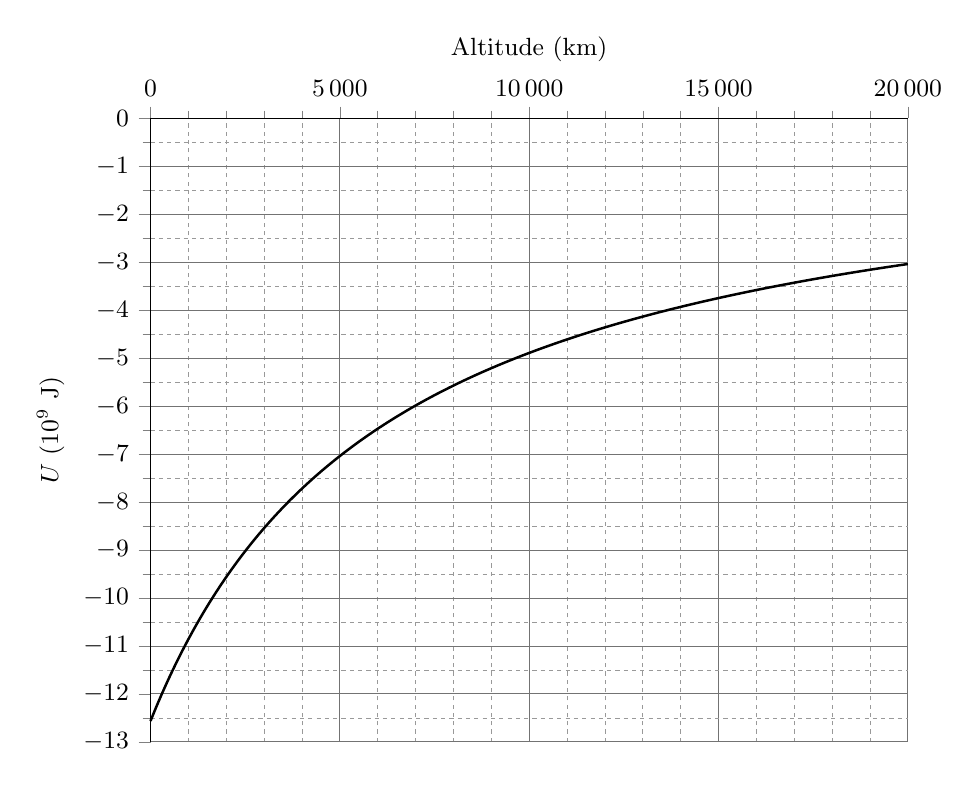
\begin{tikzpicture}
    \begin{axis}[width=112mm, height=95mm,
        axis x line*=top, axis y line*=left, axis line style={line width=0.6pt},
        xmin=0, xmax=20000, ymin=-13, ymax=0,
        xtick={0,5000,10000,15000,20000}, ytick={-13,-12,...,0},
        minor x tick num=4, minor y tick num=1,
        grid=both, major grid style={black!55, line width=0.35pt},
        minor grid style={black!40, line width=0.25pt, dash pattern=on 1.5pt off 1.5pt},
        tick align=outside, tick label style={font=\small},
        xticklabel style={/pgf/number format/1000 sep={\,}},
        scaled ticks=false, enlargelimits=false, clip=false,
        xlabel={Altitude (km)}, ylabel={$U$ ($10^{9}$ J)},
        xlabel style={font=\small}, ylabel style={font=\small}]
      \addplot[black, line width=0.9pt, domain=0:20000, samples=120, smooth]
        {-6.67e-11*6.0e24*200/((6371+x)*1000)/1e9};
    \end{axis}
  \end{tikzpicture}
\end{center}
What is the change in gravitational potential energy of the satellite when its altitude is
increased from \qty{2000}{km} to \qty{12000}{km}?
\opts{\qty{-1.4e10}{J}}{\qty{-5.2e9}{J}}{\qty[retain-explicit-plus]{+5.2e9}{J}}
  {\qty[retain-explicit-plus]{+1.4e10}{J}}
\end{quizq}

% ---- Q25 (force falls to one-ninth: what happens to U)
\Needspace{14\baselineskip}
\begin{quizq}{}
A satellite is moved to a new orbit where the gravitational force on it is one-ninth of its
initial value.

What is the gravitational potential energy of the satellite in its new orbit? (Both values of
potential energy are negative.)
\opts{One-third of the initial value.}{One-ninth of the initial value.}
  {Three times the initial value.}{Nine times the initial value.}
\end{quizq}

% ---- Q26 (escape velocity: distance matters, mass does not)
\Needspace{15\baselineskip}
\begin{quizq}{}
A space probe of mass $m$ is at a distance $8r$ from the centre of Earth. The escape velocity for
this probe is $v$.

A second probe, of mass $2m$, is at a distance $2r$ from the centre of Earth. What is the escape
velocity for the second probe?
\opts{$\dfrac{v}{2}$}{$\sqrt{2}\,v$}{$2v$}{$4v$}
\end{quizq}

% ---- Q27 (rank escape velocities from a data table)
\Needspace{22\baselineskip}
\begin{quizq}{}
Consider the information about three planets shown in the table.

\begin{center}
  \renewcommand\arraystretch{1.7}
  \begin{tabular}{|>{\centering\arraybackslash}p{20mm}|>{\centering\arraybackslash}p{30mm}%
      |>{\centering\arraybackslash}p{30mm}|>{\centering\arraybackslash}p{50mm}|}
    \hline
    \textbf{Planet} & \textbf{Mass (kg)} & \textbf{Diameter (km)} &
      \textbf{Distance from its star ($\times 10^{6}$ km)}\\ \hline
    X & \num{2.0e24} & \num{8000} & 80\\ \hline
    Y & \num{6.0e24} & \num{20000} & 150\\ \hline
    Z & \num{1.0e24} & \num{3000} & 300\\ \hline
  \end{tabular}
\end{center}
Based on this information, which choice best predicts the relative size of the escape velocity
for each planet?
\opts{Z > Y > X}{Y > X > Z}{Z > X > Y}{X > Y > Z}
\end{quizq}

% ---- Q28 (escape velocity from Mercury)
\Needspace{12\baselineskip}
\begin{quizq}{}
Mercury has a mass of \qty{3.30e23}{kg} and a radius of \qty{2.44e6}{m}. What is the escape velocity
from the surface of Mercury?
\opts{\qty{3.00e3}{m.s^{-1}}}{\qty{4.25e3}{m.s^{-1}}}{\qty{1.34e5}{m.s^{-1}}}
  {\qty{1.80e7}{m.s^{-1}}}
\end{quizq}

% ---- Q29 (U of a mass moved along the line between two identical planets)
% Correct curve: U = -k (1/x + 1/(3 - x)) for x from 0.25 to 2.75, with k = 0.45.
\Needspace{40\baselineskip}
\begin{quizq}{}
A small mass is positioned close to one of two identical planets, P and Q, as shown.

The mass is then moved at a steady speed along the straight line from $S$ to $F$.
\begin{center}
  \begin{tikzpicture}
    \fill[black!12] (0,0) circle (0.55); \draw (0,0) circle (0.55);
    \node at (0,0) {\textit{P}};
    \fill[black!12] (6,0) circle (0.55); \draw (6,0) circle (0.55);
    \node at (6,0) {\textit{Q}};
    \draw[displacement] (0.95,0) -- (5.05,0);
    \fill (0.95,0) circle (2pt) node[above=2pt] {$S$};
    \fill (5.05,0) circle (1.5pt) node[above=2pt] {$F$};
  \end{tikzpicture}
\end{center}
Which graph best represents the gravitational potential energy, $U$, of the mass during this
movement?
\gridopts{%
  \begin{tikzpicture}
    \draw[line width=0.6pt] (0,0) -- (3.2,0); \draw[line width=0.6pt] (0,0) -- (0,-2.3);
    \node[above] at (1.6,0) {Time}; \node[left] at (0,-1.15) {$U$};
    \draw[line width=0.8pt] (0.25,-1.3) -- (2.75,-1.3);
  \end{tikzpicture}}
  {%
  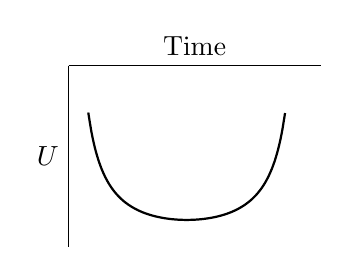
\begin{tikzpicture}
    \draw[line width=0.6pt] (0,0) -- (3.2,0); \draw[line width=0.6pt] (0,0) -- (0,-2.3);
    \node[above] at (1.6,0) {Time}; \node[left] at (0,-1.15) {$U$};
    \draw[line width=0.8pt, domain=0.25:2.75, samples=60, smooth]
      plot (\x, {-2.56 + 0.45*(1/\x + 1/(3-\x))});
  \end{tikzpicture}}
  {%
  \begin{tikzpicture}
    \draw[line width=0.6pt] (0,0) -- (3.2,0); \draw[line width=0.6pt] (0,0) -- (0,-2.3);
    \node[above] at (1.6,0) {Time}; \node[left] at (0,-1.15) {$U$};
    \draw[line width=0.8pt] (0.25,-1.96) -- (2.75,-0.6);
  \end{tikzpicture}}
  {%
  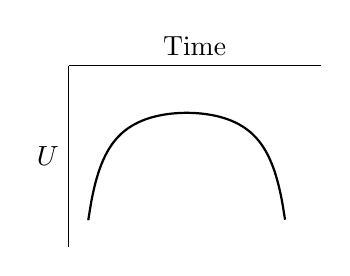
\begin{tikzpicture}
    \draw[line width=0.6pt] (0,0) -- (3.2,0); \draw[line width=0.6pt] (0,0) -- (0,-2.3);
    \node[above] at (1.6,0) {Time}; \node[left] at (0,-1.15) {$U$};
    \draw[line width=0.8pt, domain=0.25:2.75, samples=60, smooth]
      plot (\x, {-0.45*(1/\x + 1/(3-\x))});
  \end{tikzpicture}}
\end{quizq}

% ---- Q30 (minimum energy to move to a higher orbit)
\Needspace{14\baselineskip}
\begin{quizq}{}
An \qty{800}{kg} satellite is moved from a circular orbit of radius \qty{7.0e6}{m} to a circular
orbit of radius \qty{2.1e7}{m} around Earth. The total energy of a satellite in a circular orbit is
$E = -\dfrac{GMm}{2r}$.

What is the minimum energy that must be supplied to the satellite?
\opts{\qty{7.6e9}{J}}{\qty{1.5e10}{J}}{\qty{3.0e10}{J}}{\qty{4.6e10}{J}}
\end{quizq}

\end{document}
